\begin{tikzpicture}
  \coordinate (bl) at (0, 0);
  \coordinate (br) at (6, 0);
  \coordinate (tr) at (6, 7);
  \coordinate (tl) at (0, 7);
  \coordinate (x) at (3, 3.5);
  \coordinate[label=above:$\mu$] (mu) at (4, 4.5);
  \coordinate[label=right:$B$] (blab) at (6, 4.5);
  \coordinate (owtr) at (6, 6.5);
  \coordinate (owbr) at (6, 2.5);
  \coordinate (muh) at (2, 2.5);
  \coordinate (iwbl) at (0, 0.5);
  \coordinate (iwtl) at (0, 4.5);

  \coordinate (xp1) at (3, 4.5);
  \coordinate (xp2) at (5.5, 4);
  \coordinate (xp1h) at (3.5, 4);
  \coordinate (xp2h) at (5, 4.5);

  \node at (mu)[circle,fill,inner sep=1pt]{};

  \draw[fill=gray, fill opacity=0.2] (mu) to (owtr) to (owbr) -- cycle;

  \draw (mu) to (x);

  \node at (x)[circle,fill,inner sep=1pt,label=above:$X_B$]{};

  \only<-3>{

    \draw[fill=gray, fill opacity=0.2] (muh) to (iwbl) to (iwtl) -- cycle;
    \node at (muh)[circle,fill,inner sep=1pt, label=below:$\widetilde\mu$]{};
    \draw (x) to (muh);
    \coordinate[label=left:$\widetilde B$] (bhlab) at (0, 2.5);
    
  }


  \only<2>{
    \draw[out=30, in=-150] (bhlab) to (muh);

  }
  \onslide<2->{
    \draw[out=-30, in=150] (mu) to (blab);
  }

  \onslide<2>{
    \coordinate[label=above:$\Sigma_{min}$] (0) at (5.25, 4.5);
    \coordinate[label=below:$\widetilde \Sigma_{min}$] (0) at (0.75, 2.5);
  }

  \onslide<3->{
    \node at (xp1) [circle,fill,inner sep=1pt, label=above:$X_1'$]{};
    \node at (xp2) [circle,fill,inner sep=1pt, label=below:$X_2'$]{};
  }

  \onslide<4>{
    \draw[->] (xp1) to (xp1h);
    \draw[->] (xp2) to (xp2h);
  }

  \onslide<5->{
    \node at (xp1h) [circle,fill,inner sep=1pt,label=below right:$\overline{X_1'}$]{};
    \node at (xp2h) [circle,fill,inner sep=1pt,label=above:$\overline{X_2'}$]{};
  }



\end{tikzpicture}
